\documentclass[aspectratio=169,10pt]{beamer}
% Техническая презентация: lualatex presentation.tex
\usepackage{fontspec}
\usepackage{babel}
\babelprovide[import,main]{russian}
\babelprovide[import]{english}
\setsansfont{DejaVu Sans}
\setmonofont{DejaVu Sans Mono}
\babelfont{rm}{DejaVu Serif}
\usepackage{graphicx}
\usepackage{xcolor}
\usepackage{listings}
\usepackage{array}
\definecolor{Accent}{HTML}{2457A7}
\definecolor{Text}{HTML}{202733}
\definecolor{Muted}{HTML}{667085}
\definecolor{Line}{HTML}{D9DEE7}
\definecolor{Panel}{HTML}{F3F5F8}
\definecolor{Positive}{HTML}{22705A}
\definecolor{Negative}{HTML}{A23C43}
\usetheme{default}
\setbeamertemplate{navigation symbols}{}
\setbeamertemplate{itemize items}[circle]
\setbeamercolor{normal text}{fg=Text,bg=}
\setbeamercolor{frametitle}{fg=Text,bg=}
\setbeamercolor{structure}{fg=Accent}
\setbeamercolor{itemize item}{fg=Accent}
\setbeamercolor{footline}{fg=Muted,bg=}
\setbeamersize{text margin left=0.85cm,text margin right=0.85cm}
\setbeamerfont{frametitle}{size=\Large,series=\bfseries}
\setbeamerfont{normal text}{size=\small}
\setbeamerfont{footline}{size=\scriptsize}
\setbeamertemplate{frametitle}{%
  \vspace{0.22cm}\insertframetitle\par
  \vspace{0.07cm}{\color{Accent}\rule{\textwidth}{0.65pt}}\vspace{0.09cm}%
}
\setbeamertemplate{footline}{%
  \hfill{\usebeamerfont{footline}\insertframenumber\hspace{0.80cm}}\vspace{0.25cm}%
}
\newcommand{\muted}[1]{{\color{Muted}\footnotesize #1}}
\newcommand{\smallpanel}[2]{%
  \fcolorbox{Line}{Panel}{%
    \parbox[c][1.54cm][c]{0.92\linewidth}{\centering%
      \textbf{#1}\par\vspace{0.14cm}{\footnotesize #2}%
    }%
  }%
}
\newcommand{\statusline}[1]{\par\vfill\muted{#1}}
\lstset{
  basicstyle=\ttfamily\scriptsize,
  backgroundcolor=\color{Panel},
  frame=single,
  rulecolor=\color{Line},
  breaklines=true,
  columns=fullflexible,
  keepspaces=true,
  showstringspaces=false,
  literate={_}{{\_}}1
}
\begin{document}
\begin{frame}[plain]
  \vfill
  {\color{Accent}\rule{0.12\textwidth}{2pt}\par}\vspace{0.42cm}
  {\LARGE\bfseries AutoSystemDesign\par}\vspace{0.25cm}
  {\Large От бизнес-требований к проверяемой модели\par}
  {\Large архитектуры микросервисной системы\par}
  \vspace{0.70cm}
  {\normalsize Дичковский Владимир\par}
  \vfill
\end{frame}

\begin{frame}{Какую задачу решает инструмент}
  \vspace{0.32cm}
  \begin{columns}[T,onlytextwidth]
    \column{0.47\textwidth}
      {\large\bfseries Проблема}\par\vspace{0.23cm}
      \begin{itemize}
        \setlength{\itemsep}{0.19cm}
        \item В BRD описаны функции и ограничения, а не компоненты.
        \item Архитектор вручную переводит требования в схемы.
        \item Согласованность C4, сценариев и API приходится проверять.
      \end{itemize}
    \column{0.47\textwidth}
      {\large\bfseries Подход}\par\vspace{0.23cm}
      \begin{itemize}
        \setlength{\itemsep}{0.19cm}
        \item LLM предлагает структурированную модель.
        \item Доменный код проверяет её правилами.
        \item Из одной модели строятся связанные артефакты.
      \end{itemize}
  \end{columns}
  \statusline{Это первая архитектурная гипотеза для ревью, а не автоматическое утверждение проекта.}
\end{frame}

\begin{frame}{Вход: один BRD заказчика}
  \muted{Демонстрационный фрагмент BRD интернет-магазина}
  \vspace{0.18cm}
  \begin{columns}[T,onlytextwidth]
    \column{0.55\textwidth}
      \fcolorbox{Line}{Panel}{\parbox[c][4.0cm][c]{0.91\linewidth}{%
        \textbf{Функциональные требования}\par\vspace{0.18cm}
        \begin{itemize}
          \setlength{\itemsep}{0.14cm}
          \item Корзина и подтверждение заказа.
          \item Проверка остатков и расчёт цены.
          \item Оплата, создание заказа, уведомление.
          \item Просмотр статуса заказа покупателем.
        \end{itemize}
      }}
    \column{0.42\textwidth}
      \fcolorbox{Line}{Panel}{\parbox[c][4.0cm][c]{0.88\linewidth}{%
        \textbf{Нефункциональные требования}\par\vspace{0.18cm}
        \begin{itemize}
          \setlength{\itemsep}{0.17cm}
          \item Обычно: 120 запросов/с
          \item В пике: 400 запросов/с
          \item p95 не выше 300 мс
          \item Доступность: 99,9\%
        \end{itemize}
      }}
  \end{columns}
  \statusline{BRD — исходные бизнес-формулировки. Состав сервисов пока не задан.}
\end{frame}

\begin{frame}{Результат извлечения: требования}
  \muted{Наглядный пример структурирования BRD; это не лог конкретного запуска LLM}
  \vspace{0.14cm}
  \begin{columns}[T,onlytextwidth]
    \column{0.53\textwidth}
      {\large\bfseries Функциональные}\par\vspace{0.10cm}
      \begin{itemize}
        \setlength{\itemsep}{0.17cm}
        \item FR-01: оформление заказа
        \item FR-02: проверка наличия товаров
        \item FR-03: оплата и подтверждение
        \item FR-04: просмотр статуса
      \end{itemize}
    \column{0.43\textwidth}
      {\large\bfseries Нефункциональные}\par\vspace{0.10cm}
      \begin{itemize}
        \setlength{\itemsep}{0.17cm}
        \item Нагрузка: 120 / 400 RPS
        \item Целевое p95: 300 мс
        \item Доступность: 99,9\%
      \end{itemize}
  \end{columns}
  \vspace{0.36cm}
  \fcolorbox{Line}{Panel}{\parbox{0.96\linewidth}{%
    {\footnotesize\textbf{След происхождения:} для каждого значения сохраняется цитата BRD; конфликтующие формулировки фиксируются отдельно.}%
  }}
\end{frame}

\begin{frame}{Извлечение не означает безусловного доверия LLM}
  \vspace{0.34cm}
  \begin{columns}[T,onlytextwidth]
    \column{0.49\textwidth}
      {\large\bfseries Двухэтапная проверка}\par\vspace{0.18cm}
      \begin{enumerate}
        \setlength{\itemsep}{0.22cm}
        \item LLM выделяет требование и цитату.
        \item Код сверяет цитату с BRD.
        \item LLM сопоставляет подтверждённое требование с полями модели.
        \item Значения ещё раз проверяются по источнику.
      \end{enumerate}
    \column{0.47\textwidth}
      {\large\bfseries Сомнительные данные}\par\vspace{0.18cm}
      \begin{itemize}
        \setlength{\itemsep}{0.22cm}
        \item Неподтверждённые числа исключаются.
        \item Противоречия сохраняются для человека.
        \item Отсутствующие данные не придумываются.
      \end{itemize}
  \end{columns}
  \statusline{Пример неоднозначности BRD: доставка письма за 10 секунд или до 2 минут в пике? Решение нужно уточнить.}
\end{frame}

\begin{frame}{Архитектура конвейера и зависимости этапов}
  \vspace{0.42cm}
  \centering
  \fcolorbox{Line}{Panel}{\parbox[c][0.75cm][c]{0.48\textwidth}{\centering\textbf{BRD → требования → сценарий}}}
  \par\vspace{0.10cm}{\color{Accent}\Large$\downarrow$}\par\vspace{0.08cm}
  \fcolorbox{Line}{Panel}{\parbox[c][0.70cm][c]{0.48\textwidth}{\centering\textbf{C4: граф архитектуры}}}
  \par\vspace{0.14cm}
  \begin{columns}[c,onlytextwidth]
    \column{0.47\textwidth}
      \centering{\color{Accent}\Large$\downarrow$}\par
      \smallpanel{Performance}{Расчёт из C4 и нагрузки}
    \column{0.47\textwidth}
      \centering{\color{Accent}\Large$\downarrow$}\par
      \smallpanel{Sequence}{Сценарии по функциям BRD}
  \end{columns}
  \vspace{0.13cm}
  {\color{Accent}\Large$\downarrow$}\par
  \fcolorbox{Line}{Panel}{\parbox[c][0.70cm][c]{0.48\textwidth}{\centering\textbf{API: OpenAPI + Swagger UI}}}
  \statusline{Performance зависит от C4; API опирается на C4 и Sequence.}
\end{frame}

\begin{frame}{Как LLM превращается в проверяемый генератор}
  \begin{columns}[T,onlytextwidth]
    \column{0.53\textwidth}
      {\large\bfseries Генерация}\par\vspace{0.18cm}
      \begin{itemize}
        \setlength{\itemsep}{0.18cm}
        \item LiteLLM: единая точка работы с моделями.
        \item LLM возвращает структурированный ответ.
        \item Pydantic преобразует его в типизированную доменную модель.
        \item Код PlantUML строит отдельный рендерер, не сама LLM.
      \end{itemize}
    \column{0.43\textwidth}
      {\large\bfseries Если нарушены правила}\par\vspace{0.18cm}
      \begin{itemize}
        \setlength{\itemsep}{0.18cm}
        \item Ошибки разбора и доменной проверки возвращаются модели.
        \item Модель исправляет ответ.
        \item Число попыток ограничено.
      \end{itemize}
  \end{columns}
  \statusline{Принцип: генеративная модель предлагает, детерминированные валидаторы принимают или отклоняют.}
\end{frame}

\begin{frame}{C4: не картинка, а модель предметной области}
  \vspace{0.23cm}
  \begin{columns}[T,onlytextwidth]
    \column{0.47\textwidth}
      {\large\bfseries Типы компонентов}\par\vspace{0.14cm}
      \begin{itemize}
        \setlength{\itemsep}{0.15cm}
        \item Клиент, балансировщик
        \item Вычислительный сервис
        \item База данных и кэш
        \item Брокер сообщений
      \end{itemize}
    \column{0.49\textwidth}
      {\large\bfseries Параметры модели}\par\vspace{0.14cm}
      \begin{itemize}
        \setlength{\itemsep}{0.15cm}
        \item Реплики и лимит параллелизма
        \item Время обработки и разброс
        \item Размер очереди и стоимость
        \item Протокол и тип маршрутизации связи
      \end{itemize}
  \end{columns}
  \vspace{0.28cm}
  \fcolorbox{Line}{Panel}{\parbox{0.96\linewidth}{%
    {\footnotesize\textbf{Зачем:} одна и та же модель нужна и для рисования диаграммы, и для расчёта нагрузки и правил валидации.}%
  }}
\end{frame}

\begin{frame}{Валидаторы C4: три уровня проверки}
  \vspace{0.25cm}
  \begin{columns}[T,onlytextwidth]
    \column{0.31\textwidth}
      \smallpanel{Структура}{Уникальные ID, допустимые связи, отсутствие циклов}
    \column{0.31\textwidth}
      \smallpanel{Семантика}{Поставщик и потребитель брокера, путь мимо кэша}
    \column{0.31\textwidth}
      \smallpanel{Расчёты}{Поток RPS, пропускная способность, насыщение}
  \end{columns}
  \vspace{0.70cm}
  \begin{columns}[T,onlytextwidth]
    \column{0.47\textwidth}
      {\color{Positive}\textbf{Допустимо}}\par\vspace{0.13cm}
      Клиент $\rightarrow$ API $\rightarrow$ БД
    \column{0.47\textwidth}
      {\color{Negative}\textbf{Недопустимо}}\par\vspace{0.13cm}
      Клиент $\rightarrow$ БД напрямую
  \end{columns}
  \statusline{Онтология допустимых связей ограничивает пространство решений, которые может предложить LLM.}
\end{frame}

\begin{frame}{Пример: диаграмма компонентов C4}
  \centering
  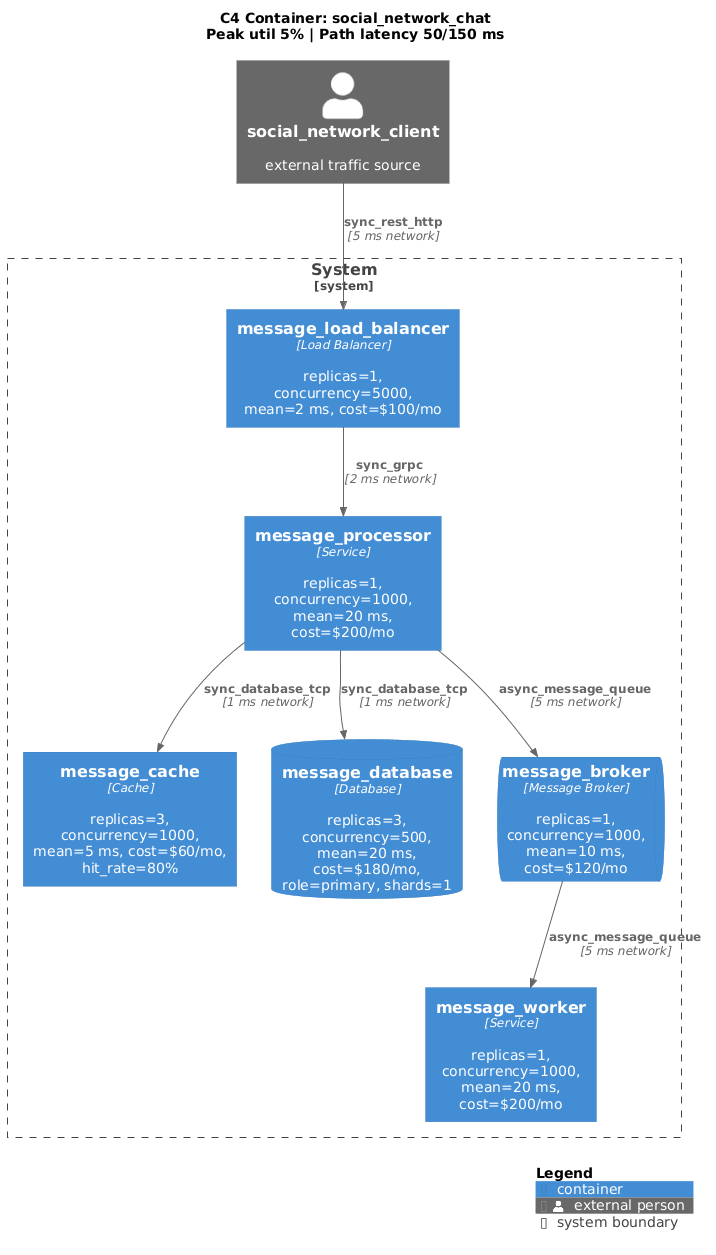
\includegraphics[width=0.99\textwidth,height=0.79\textheight,keepaspectratio]{images/c4_example_2.png}
  \statusline{Иллюстрация из репозитория. Позже будет заменена результатом единого BRD-прогона.}
\end{frame}

\begin{frame}{Связи: протокол влияет на смысл графа}
  \vspace{0.25cm}
  \begin{columns}[T,onlytextwidth]
    \column{0.48\textwidth}
      {\large\bfseries Контракт связи}\par\vspace{0.13cm}
      \begin{itemize}
        \setlength{\itemsep}{0.17cm}
        \item HTTP, gRPC, TCP или очередь сообщений
        \item Синхронный или асинхронный обмен
        \item Альтернативный маршрут либо fan-out
      \end{itemize}
    \column{0.48\textwidth}
      {\large\bfseries Почему это важно}\par\vspace{0.13cm}
      \begin{itemize}
        \setlength{\itemsep}{0.17cm}
        \item Разные пути по-разному получают RPS.
        \item Асинхронные ветви не добавляются к задержке клиентского ответа.
        \item Очередь и кэш меняют путь обработки.
      \end{itemize}
  \end{columns}
  \statusline{Это модель обмена и распределения трафика, а не просто подписи на стрелках.}
\end{frame}

\begin{frame}{Sequence: от функционального требования к сценарию}
  \vspace{0.22cm}
  \begin{columns}[T,onlytextwidth]
    \column{0.49\textwidth}
      {\large\bfseries Построение}\par\vspace{0.12cm}
      \begin{itemize}
        \setlength{\itemsep}{0.18cm}
        \item Каталог бизнес-ролей.
        \item Сценарий взаимодействия на каждое функциональное требование.
        \item Участники ссылаются на компоненты C4.
      \end{itemize}
    \column{0.47\textwidth}
      {\large\bfseries Проверка}\par\vspace{0.12cm}
      \begin{itemize}
        \setlength{\itemsep}{0.18cm}
        \item Существующие участники и связи.
        \item Согласованность ролей и клиента.
        \item Асинхронность уведомлений и событий.
      \end{itemize}
  \end{columns}
  \statusline{Последовательность объясняет поведение архитектуры, которое не видно на статической C4.}
\end{frame}

\begin{frame}{Пример: диаграмма последовательностей}
  \centering
  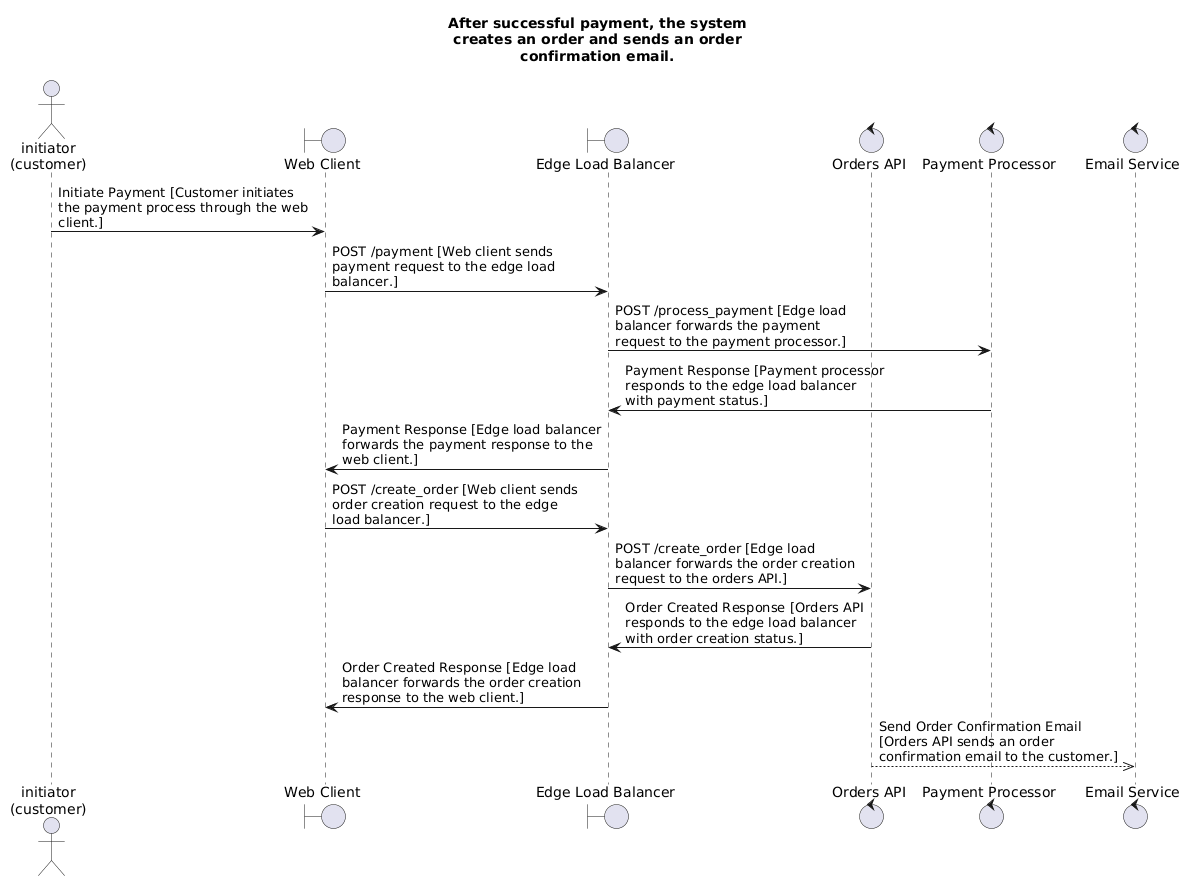
\includegraphics[width=0.99\textwidth,height=0.79\textheight,keepaspectratio]{images/sequence_example_3.png}
  \statusline{Иллюстрация из репозитория; связь с выбранным BRD ещё будет проверена на едином прогоне.}
\end{frame}

\begin{frame}{REST API: контракт строится после C4 и Sequence}
  \vspace{0.25cm}
  \begin{columns}[T,onlytextwidth]
    \column{0.49\textwidth}
      {\large\bfseries Что генерируется}\par\vspace{0.13cm}
      \begin{itemize}
        \setlength{\itemsep}{0.18cm}
        \item Операции, методы и маршруты
        \item Параметры, запросы и ответы
        \item Связь операций с требованиями и компонентами
      \end{itemize}
    \column{0.47\textwidth}
      {\large\bfseries Что проверяется}\par\vspace{0.13cm}
      \begin{itemize}
        \setlength{\itemsep}{0.18cm}
        \item Уникальность операций
        \item Отсутствие коллизий маршрутов
        \item Согласованность ссылок и схем
      \end{itemize}
  \end{columns}
  \statusline{OpenAPI описывает машинный контракт. Swagger UI делает его удобным для просмотра людьми.}
\end{frame}

\begin{frame}{Пример: Swagger UI}
  \centering
  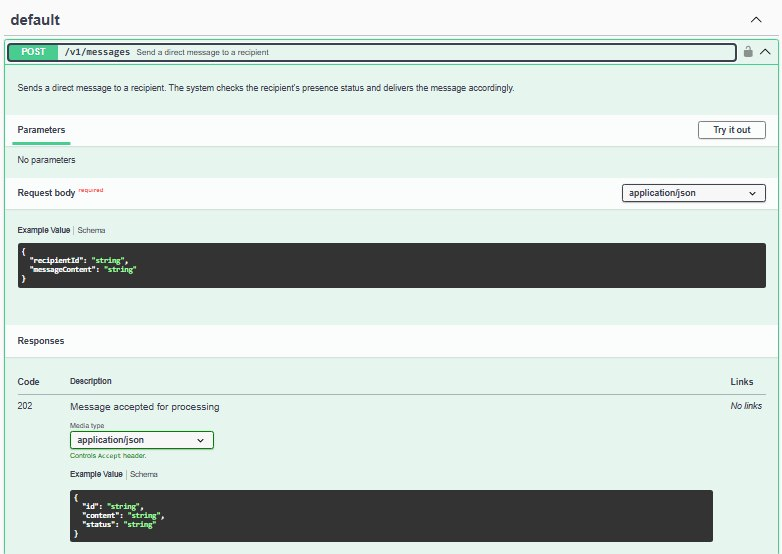
\includegraphics[width=0.99\textwidth,height=0.79\textheight,keepaspectratio]{images/swagger_example_2.png}
  \statusline{Существующий скриншот. Для финальной демонстрации нужен Swagger от того же BRD.}
\end{frame}

\begin{frame}[fragile]{Пример: фрагмент OpenAPI JSON}
  \muted{Сокращённый иллюстративный контракт для оформления заказа, не фактический файл генерации}
  \vspace{0.12cm}
  \begin{lstlisting}[basicstyle=\ttfamily\scriptsize]
{
  "openapi": "3.1.0",
  "info": {
    "title": "Checkout API",
    "version": "1.0.0"
  },
  "paths": {
    "/orders": {
      "post": {
        "operationId": "createOrder",
        "summary": "Create a customer order",
        "responses": {
          "201": { "description": "Order created" },
          "409": { "description": "Item out of stock" }
        }
      }
    }
  }
}
  \end{lstlisting}
\end{frame}

\begin{frame}{Анализ производительности: что считаем}
  \vspace{0.30cm}
  \begin{columns}[T,onlytextwidth]
    \column{0.49\textwidth}
      {\large\bfseries Математическая часть}\par\vspace{0.16cm}
      \begin{itemize}
        \setlength{\itemsep}{0.17cm}
        \item Распределение RPS по путям графа.
        \item Пропускная способность и загрузка узлов.
        \item Оценка ожидания в очередях и средних задержек.
      \end{itemize}
    \column{0.47\textwidth}
      {\large\bfseries Условия применимости}\par\vspace{0.16cm}
      \begin{itemize}
        \setlength{\itemsep}{0.17cm}
        \item M/M/1, M/M/c и G/G/c: модели с допущениями.
        \item Число обслуживающих каналов не равно автоматически лимиту параллелизма.
        \item Неизвестная величина остаётся неизвестной.
      \end{itemize}
  \end{columns}
  \statusline{Это аналитическая оценка модели, не нагрузочный тест и не моделирование реального кластера.}
\end{frame}

\begin{frame}{Пример: отчёт анализа производительности}
  \begin{columns}[c,onlytextwidth]
    \column{0.71\textwidth}
      \centering
      \IfFileExists{images/performance_report_checkout.png}{%
        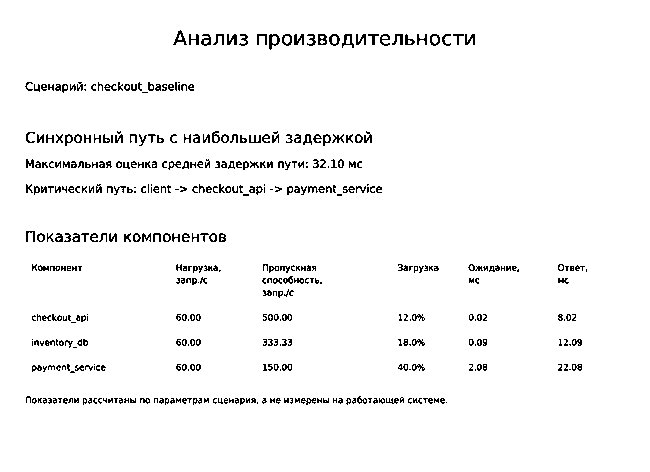
\includegraphics[width=\linewidth,height=0.72\textheight,keepaspectratio]{images/performance_report_checkout.png}%
      }{%
        \fcolorbox{Line}{Panel}{\parbox[c][4.0cm][c]{0.94\linewidth}{%
          \centering\textbf{checkout\_baseline}\par\vspace{0.25cm}
          Скриншот PDF-отчёта\par\vspace{0.20cm}
          32,10 мс: оценка средней задержки пути
        }}%
      }
    \column{0.25\textwidth}
      {\bfseries\large Пример}\par\vspace{0.18cm}
      {\small
      \textbf{60 RPS}\par\vspace{0.18cm}
      нагрузка узлов\par\vspace{0.30cm}
      \textbf{32,10 мс}\par\vspace{0.18cm}
      максимальная оценка средней задержки пути\par
      }
  \end{columns}
  \statusline{Реальный отчёт checkout\_baseline из предоставленного PDF; исходный BRD демонстрационного примера отличается.}
\end{frame}

\begin{frame}{Почему среднее время не доказывает p95}
  \vspace{0.35cm}
  \begin{columns}[T,onlytextwidth]
    \column{0.47\textwidth}
      {\large\bfseries В отчёте есть}\par\vspace{0.22cm}
      \begin{itemize}
        \setlength{\itemsep}{0.19cm}
        \item Средняя оценка ответа и ожидания.
        \item Загрузка и пропускная способность.
        \item Синхронный путь с наибольшей суммой средних задержек.
      \end{itemize}
    \column{0.47\textwidth}
      {\large\bfseries Отчёт не доказывает}\par\vspace{0.22cm}
      \begin{itemize}
        \setlength{\itemsep}{0.19cm}
        \item Соблюдение p95 или p99 по одному среднему.
        \item Поведение на реальной инфраструктуре.
        \item Потери при ограниченных очередях без модели.
      \end{itemize}
  \end{columns}
  \vspace{0.38cm}
  \fcolorbox{Line}{Panel}{\parbox{0.96\linewidth}{%
    {\small\textbf{Пример:} среднее 32,10 мс не означает, что p95 не превысит 300 мс.}%
  }}
\end{frame}

\begin{frame}{Разделение ответственности внутри системы}
  \vspace{0.20cm}
  \begin{columns}[T,onlytextwidth]
    \column{0.31\textwidth}
      \smallpanel{Domain}{Типизированные модели, инварианты, расчёты}
    \column{0.31\textwidth}
      \smallpanel{Application}{Сервисы и стадии конвейера}
    \column{0.31\textwidth}
      \smallpanel{Infrastructure}{LLM, PlantUML, Swagger, PDF}
  \end{columns}
  \vspace{0.58cm}
  \begin{itemize}
    \setlength{\itemsep}{0.19cm}
    \item Замена модели LLM не должна переписывать доменные правила.
    \item Исходники PlantUML, граф и артефакты API хранятся отдельно.
    \item Рендеринг диаграмм поддерживает PlantUML и Kroki.
  \end{itemize}
  \statusline{Результат описывается моделью, а не зависит от конкретного формата изображения.}
\end{frame}

\begin{frame}{Текущие возможности и границы}
  \vspace{0.18cm}
  \begin{columns}[T,onlytextwidth]
    \column{0.49\textwidth}
      {\large\bfseries Реализовано}\par\vspace{0.12cm}
      \begin{itemize}
        \setlength{\itemsep}{0.18cm}
        \item Извлечение требований из BRD с цитатами и проверками.
        \item C4, Sequence, OpenAPI и Swagger.
        \item Расчётный JSON-отчёт и PDF-представление.
        \item Консольный запуск конвейера.
      \end{itemize}
    \column{0.47\textwidth}
      {\large\bfseries Следующие задачи}\par\vspace{0.12cm}
      \begin{itemize}
        \setlength{\itemsep}{0.18cm}
        \item Один воспроизводимый BRD-прогон для всех демонстрационных артефактов.
        \item Удобный интерфейс загрузки BRD и просмотра результатов.
        \item Развитие проверок и независимая оценка точности.
      \end{itemize}
  \end{columns}
  \statusline{Автоматическая генерация — начало проектирования. Окончательное решение остаётся за архитектором.}
\end{frame}
\end{document}
